\documentclass[12pt]{article} % 12pt 为字号大小 UTF8
\usepackage{amssymb,amsfonts,amsmath,amsthm}
%\usepackage{fontspec,xltxtra,xunicode}
%\usepackage{times}

%----------
% 定义中文环境
%----------

\usepackage{xeCJK}

% \setCJKmainfont[BoldFont={SimHei},ItalicFont={KaiTi}]{SimSun}
% \setCJKsansfont{SimHei}
% \setCJKfamilyfont{zhsong}{SimSun}
% \setCJKfamilyfont{zhhei}{SimHei}

% \newcommand*{\songti}{\CJKfamily{zhsong}} % 宋体
% \newcommand*{\heiti}{\CJKfamily{zhhei}}   % 黑体


%----------
% 版面设置
%----------
%首段缩进
\usepackage{indentfirst}
\setlength{\parindent}{2.1em}

%行距
\renewcommand{\baselinestretch}{1.2} % 1.4倍行距

%页边距
\usepackage[a4paper]{geometry}
\geometry{verbose,
  tmargin=3cm,% 上边距
  bmargin=3cm,% 下边距
  lmargin=3cm,% 左边距
  rmargin=3cm % 右边距
}


%----------
% 其他宏包
%----------
%图形相关
\usepackage[x11names]{xcolor} % must before tikz, x11names defines RoyalBlue3
\usepackage{graphicx}
\usepackage{pstricks,pst-plot,pst-eps}
\usepackage{subfig}
\def\pgfsysdriver{pgfsys-dvipdfmx.def} % put before tikz
\usepackage{tikz}

%原文照排
\usepackage{verbatim}
\usepackage{float}

%网址
\usepackage{url}

%文本格式
\usepackage{ulem} % 用法:\uline{}下划线,\uwave{}波浪线,\sout{}删除线
\usepackage{pifont} % 用法:\ding{数字}代表数字被圈起来
\usepackage{enumitem} % 使用enumitem宏包自定义列表样式
\usepackage{hyperref} % 不仅可以帮助你插入链接,还能让这些链接在生成的PDF文档中是可点击的,提高文档的互动性,用法:\url{http://www.example.com}


%----------
% 习题与解答环境
%----------
%习题环境
\theoremstyle{definition} 
\newtheorem{problem}{题目}

%解答环境
\ifx\proof\undefined\
\newenvironment{proof}[1][\protect\proofname]{\par
\normalfont\topsep6\p@\@plus6\p@\relax
\trivlist
\itemindent\parindent
\item[\hskip\labelsep
\scshape
#1]\ignorespaces
}{%
\endtrivlist\@endpefalse
}
\fi
\renewcommand{\proofname}{\it{解答}}


%----------
% 我的自定义
%----------

\newcommand{\horrule}[1]{\rule[0.5ex]{\linewidth}{#1}} 	% Horizontal rule

\renewcommand{\refname}{参考文献}
\renewcommand{\abstractname}{\large \bf 摘\quad 要}
\renewcommand{\contentsname}{目录}
\renewcommand{\tablename}{表}
\renewcommand{\figurename}{图}

\setlength{\parskip}{0.4ex} % 段落间距

\usepackage{enumitem}
\setenumerate[1]{itemsep=0pt,partopsep=0pt,parsep=\parskip,topsep=5pt}
\setitemize[1]{itemsep=0.4ex,partopsep=0.4ex,parsep=\parskip,topsep=0.4ex}
\setdescription{itemsep=0pt,partopsep=0pt,parsep=\parskip,topsep=5pt}


%==========
% 正文部分
%==========

\begin{document}

\title{
{\normalfont\normalsize\textsc{
Peking University\\
Introduction to Database Systems, Spring 2024 \\[25pt]}}
\horrule{0.5pt}\\
\sffamily{第二章 ER模型\\课后作业}
\horrule{1.8pt}\\[20pt]
}
\author{梁昱桐\quad 2100013116\\lyt0112@outlook.com}
% \date{} % 若不需要自动插入日期,则去掉前面的注释;{ } 中也可以自定义日期格式

\begin{titlepage}
\maketitle
\vspace{30pt}

% \begin{abstract}
% \normalsize \ \ 这是中文摘要。大概写满这一页可以了。摘要又称概要、内容提要。摘要是以提供文献内容梗概为目的,不加评论和补充解释,简明、确切地记述文献重要内容的短文。其基本要素包括研究目的、方法、结果和结论。具体地讲就是研究工作的主要对象和范围,采用的手段和方法,得出的结果和重要的结论,有时也包括具有情报价值的其它重要的信息。\\[5pt]
% \indent \ \ \textbf{关键词}:图卷积神经网络,复杂网络,表示学习
% \end{abstract}

\thispagestyle{empty}
\end{titlepage}

% \tableofcontents
% \thispagestyle{empty}

\newpage
\setcounter{page}{1}

\begin{problem}
分别列举聚集、弱实体、细化/泛化的实用例子,记得不要同讲义上的相同。
说明在此时采用这些扩展表示方法的优点。
\end{problem}

\begin{proof}

\textbf{聚集示例}

\textit{场景}: 假设我们有一个图书馆管理系统,其中包括实体集“图书 (Book)”和“作者 (Author)”,以及这两个实体集之间的联系集“写作 (Writes)”。
此外,还有一个实体集“出版社 (Publisher)”与“图书 (Book)”之间存在联系集“出版 (Publishes)”。

\textit{应用}: 我们可以将“图书 (Book)”和“作者 (Author)”以及它们之间的“写作 (Writes)”联系聚集为一个高层实体集“作品 (Work)”,
然后这个“作品 (Work)”实体集再与“出版社 (Publisher)”实体集通过“出版 (Publishes)”联系发生关系。

\textit{优点}: 这样可以把有先后关系的三个实体间的联系用更加清晰的方式表述出来,
比如可以防止有的人自己出版图书并没有通过出版商出版,无法在三元关系中表示出来的情况发生。

\vspace{5mm} %5mm vertical space

\textbf{弱实体集示例}

\textit{场景}: 在一个大学数据库系统中,我们有一个“学生 (Student)”实体集,每个学生有一个独一无二的学号作为主码。
还有一个实体集“课程报告 (CourseReport)”记录了学生提交的各种课程报告,但是课程报告只有“课程”这个属性。

\textit{应用}: “课程报告 (CourseReport)”依赖于“学生 (Student)”实体集,因为每个课程报告都必须由一个特定的学生提交,
但报告本身没有足够的属性来构成一个主码。因此,“课程报告 (CourseReport)”可以被视为一个弱实体集,
它通过“提交 (Submit)”的联系与“学生 (Student)”实体集相连,这里的学号+课程名成为了弱实体集的主码,课程名是课程报告的部分码。

\textit{优点}: 如果不使用这样的方法,无法将课程报告作为主体表示出来。

\vspace{5mm} %5mm vertical space

\textbf{特化示例}

\textit{场景}: 在教育管理系统中,可以有一个通用的“人员 (Person)”实体集,它包含所有人员共有的属性,例如姓名、身份证号和地址。

\textit{应用}: 在这个系统中,根据不同的角色和职责,人员可以进一步被特化为“教师 (Teacher)”和“学生 (Student)”两个子实体。
教师实体集继承了“人员 (Person)”的所有属性,并添加了一些特有的属性,如“教师编号 (TeacherID)”、“所教科目 (Subject)”和“职称 (Title)”。
学生实体集同样继承了“人员 (Person)”的所有属性,并且增加了一些特有的属性,如“学生编号 (StudentID)”、“所在班级 (Class)”和“学籍状态 (Status)”。

\textit{优点}: 这样可以更好地组织实体集,使得对象和种类更加精确。

\vspace{5mm} %5mm vertical space

\textbf{概化示例}

\textit{场景}: 在一个公司的人力资源管理系统中,可以有“工程师 (Engineer)”、“会计 (Accountant)”和“管理人员 (Manager)”等不同实体集,

\textit{应用}: 它们都有一些共同的属性,如姓名、员工ID和地址。通过概化,我们可以将这些实体集合并为一个更高层次的“员工 (Employee)”实体集,它包含所有子集共有的属性。

\textit{优点}: 这样可以更好地组织实体集,使得系统更加清晰。在这种情况下,成员身份是重叠的、全部的。

\end{proof}

\begin{problem}
已知有如下关系模式:
\[
R1(\underline{a1},a2, a3),	R2(\underline{a3}, a4,a1) ,		R3(\underline{a5}, a6),
R4(\underline{a3},\underline{a5}, a7),	R5(\underline{a1},\underline{a3},\underline{a5}, a8)
\]

其中带下划线的属性标识为所在关系模式的主码,关系模式之间重合的属性是主外码关系,体现了实体之间的联系。
试画出相应的E-R图,使得可以从该E-R图推导出上述关系模式
\end{problem}  

\begin{proof}
观察发现$R1$和$R2$之间存在一对一的联系;$R2$和$R2$之间的联系是$R4$;$R1$、$R2$和$R3$的聚集看作一个新的实体,它拥有属性$a8$。
因此,可以画出如下的E-R图:
\begin{figure}[H]
  \centering
  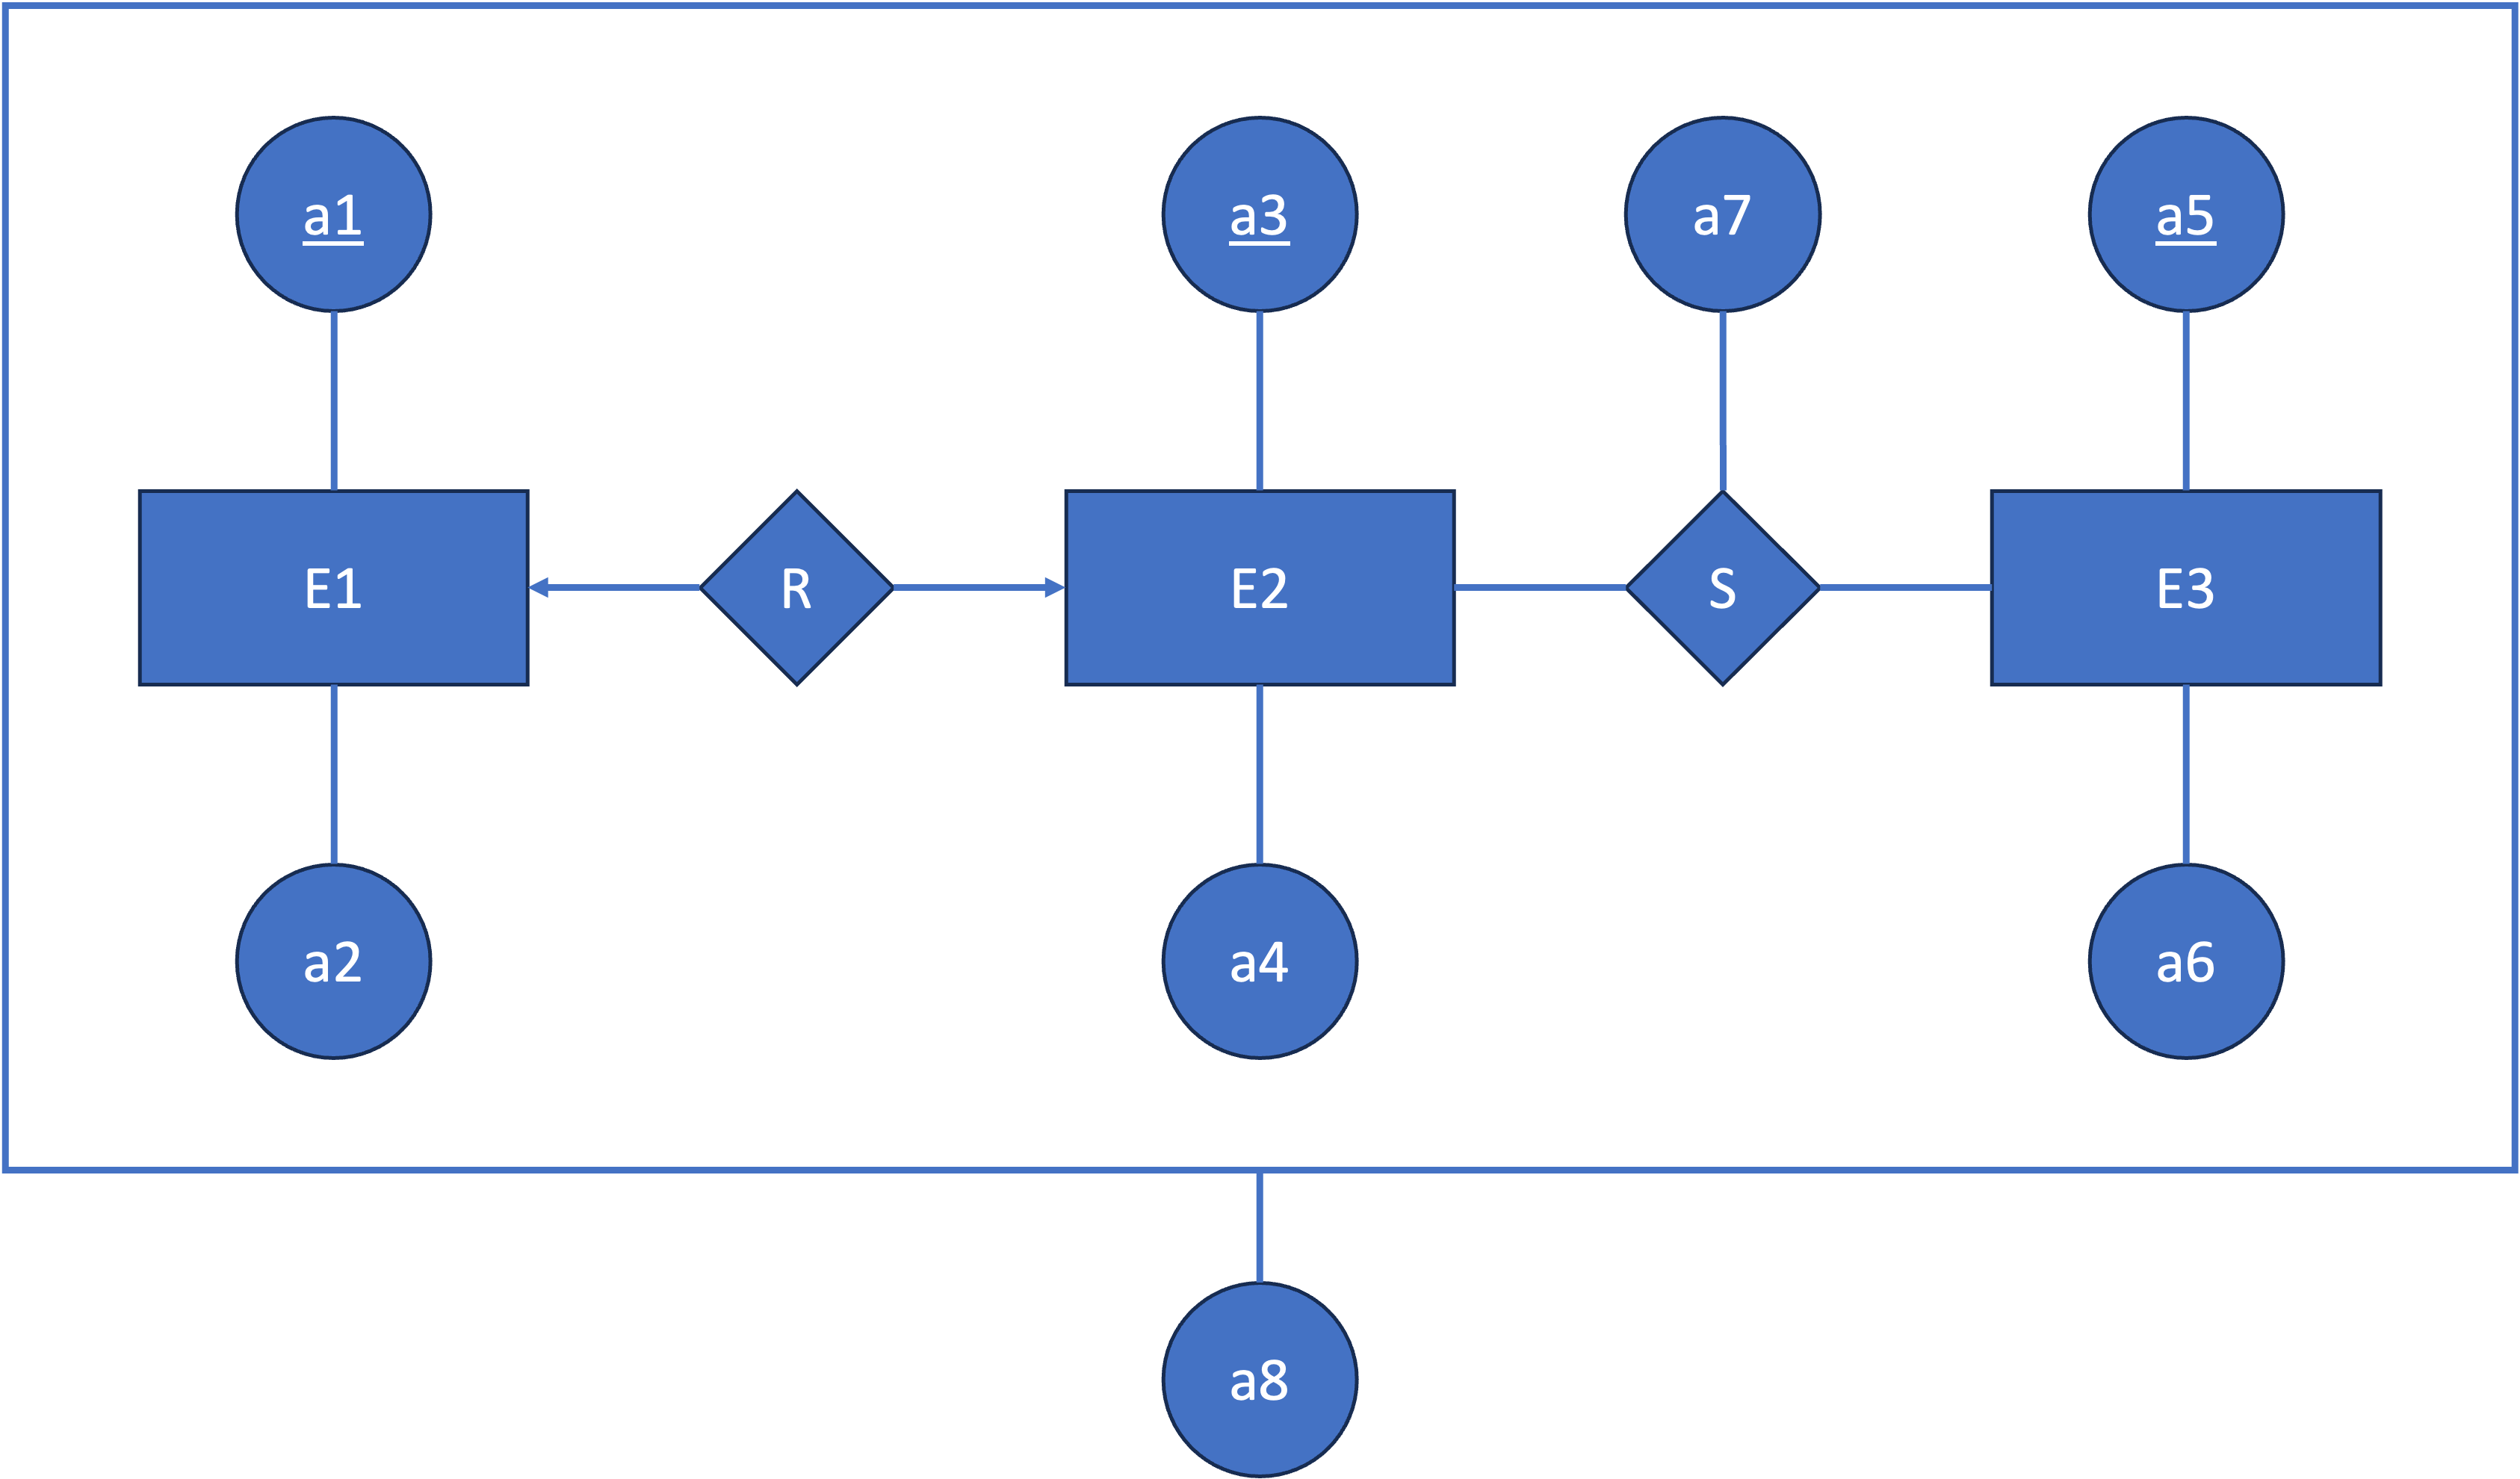
\includegraphics[width=1\textwidth]{./figs/2.png}
  \caption{题2的E-R图}
\end{figure}
\end{proof}

\begin{problem}
下面是一张NBA球员转会的汇总表格,基于这些表格中的数据,请画出合适的ER图。 
\begin{figure}[H]
  \centering
  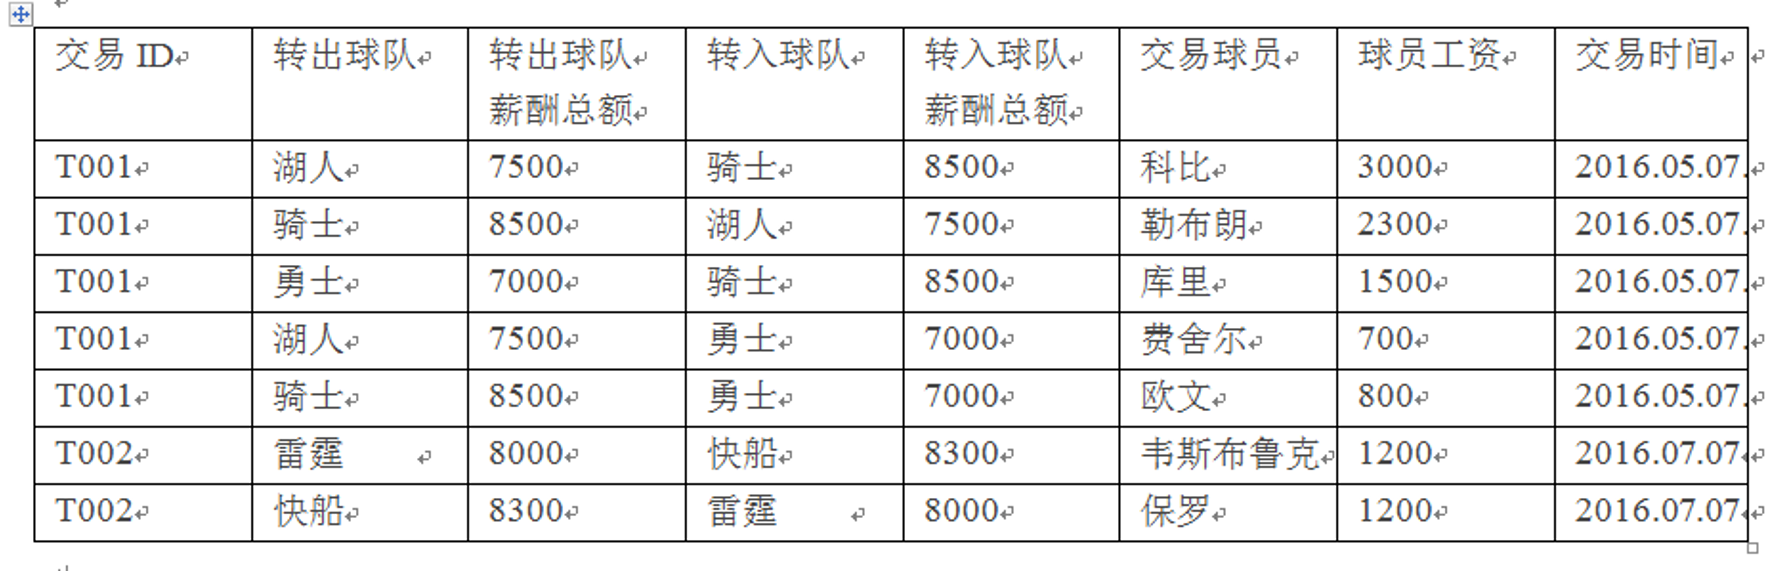
\includegraphics[width=0.8\textwidth]{./figs/3.png}
  \caption{NBA球员转会汇总表格}
\end{figure}
\end{problem}

\begin{proof}
可以画出如下的E-R图:
\begin{figure}[H]
  \centering
  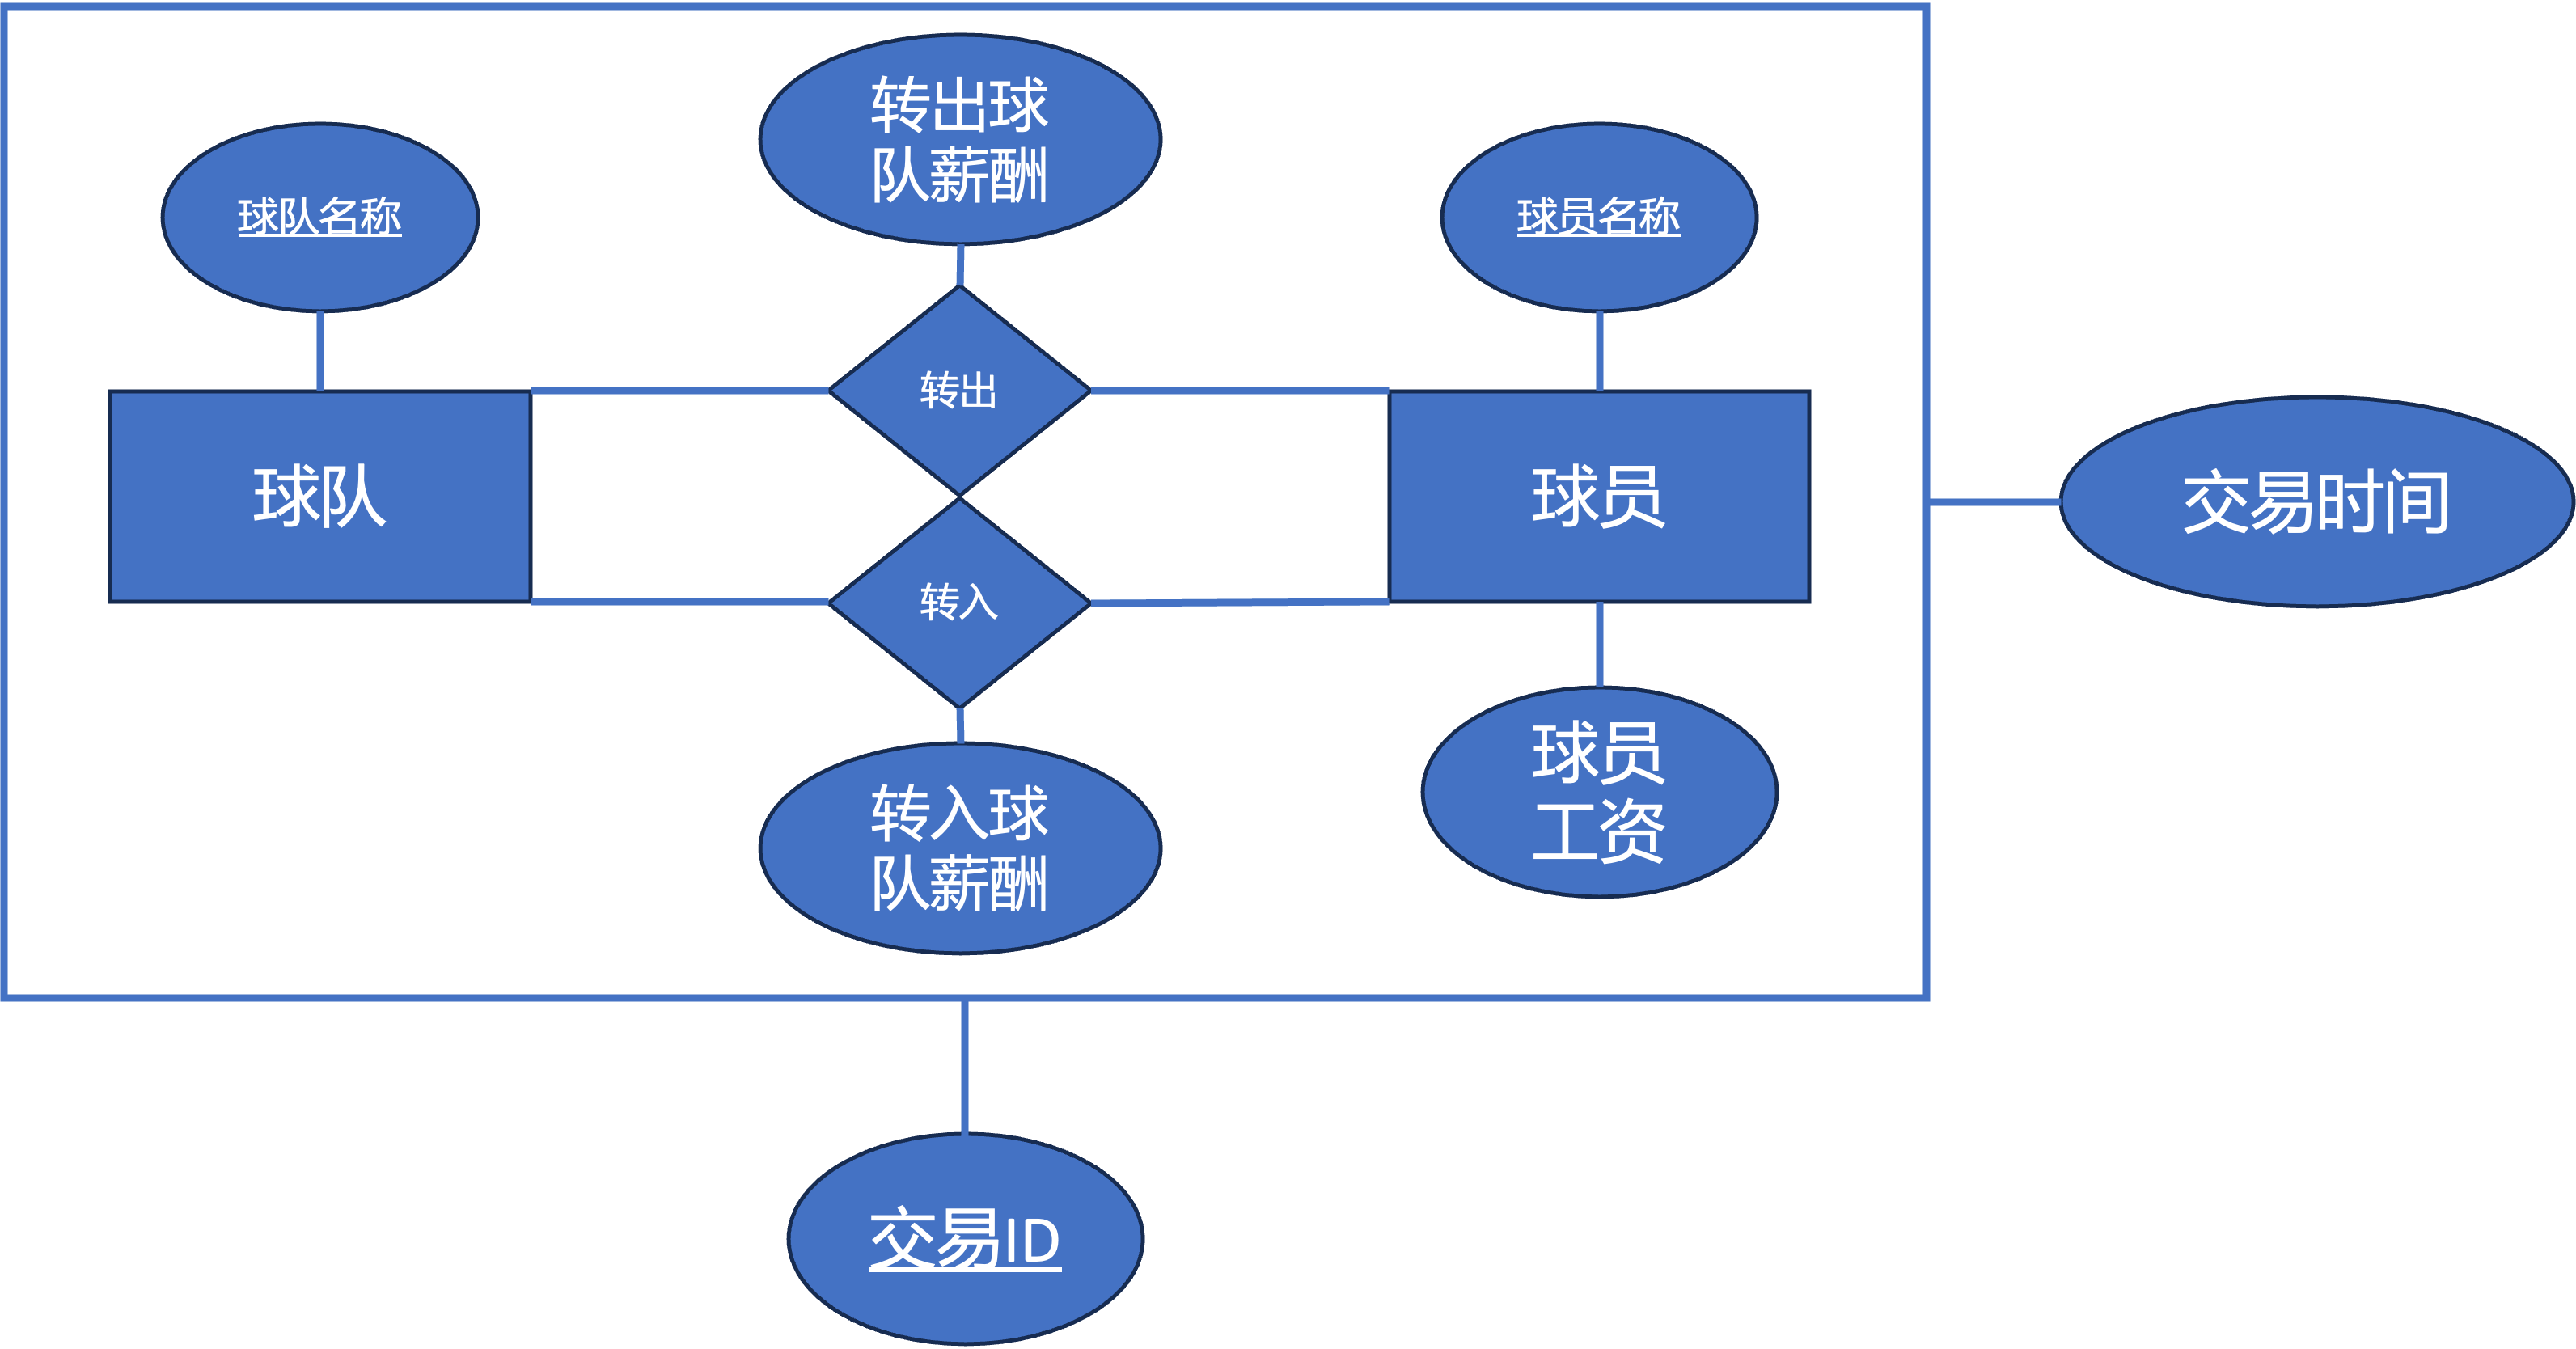
\includegraphics[width=1\textwidth]{./figs/3.1.png}
  \caption{题3的E-R图}
\end{figure}
\end{proof}

\begin{problem}
假定以下是存储微信内容的数据库相关表,请根据这些表画出微信的ER图。
\begin{itemize}
  \item 信友(\uline{信友ID},信友名,昵称,所在区域,手机号)
  \item 通讯录(\uline{信友1 ID},\uline{信友2 ID},认识方式,认识时间)
  \item 群(\uline{群ID},群名称,群类型,创建时间,群主ID)
  \item 群成员(\uline{群ID},\uline{信友ID},加入时间,引介人ID,信友群内昵称)
  \item 帖子(\uline{帖子ID},发帖信友ID,所属群ID,帖子内容,发帖时间)
  \item 短信(\uline{短信ID},发送信友ID,接受信友ID,短信时间,短信内容)
\end{itemize}
\end{problem}

\begin{proof}
可以画出如下的E-R图:
\begin{figure}[H]
  \centering
  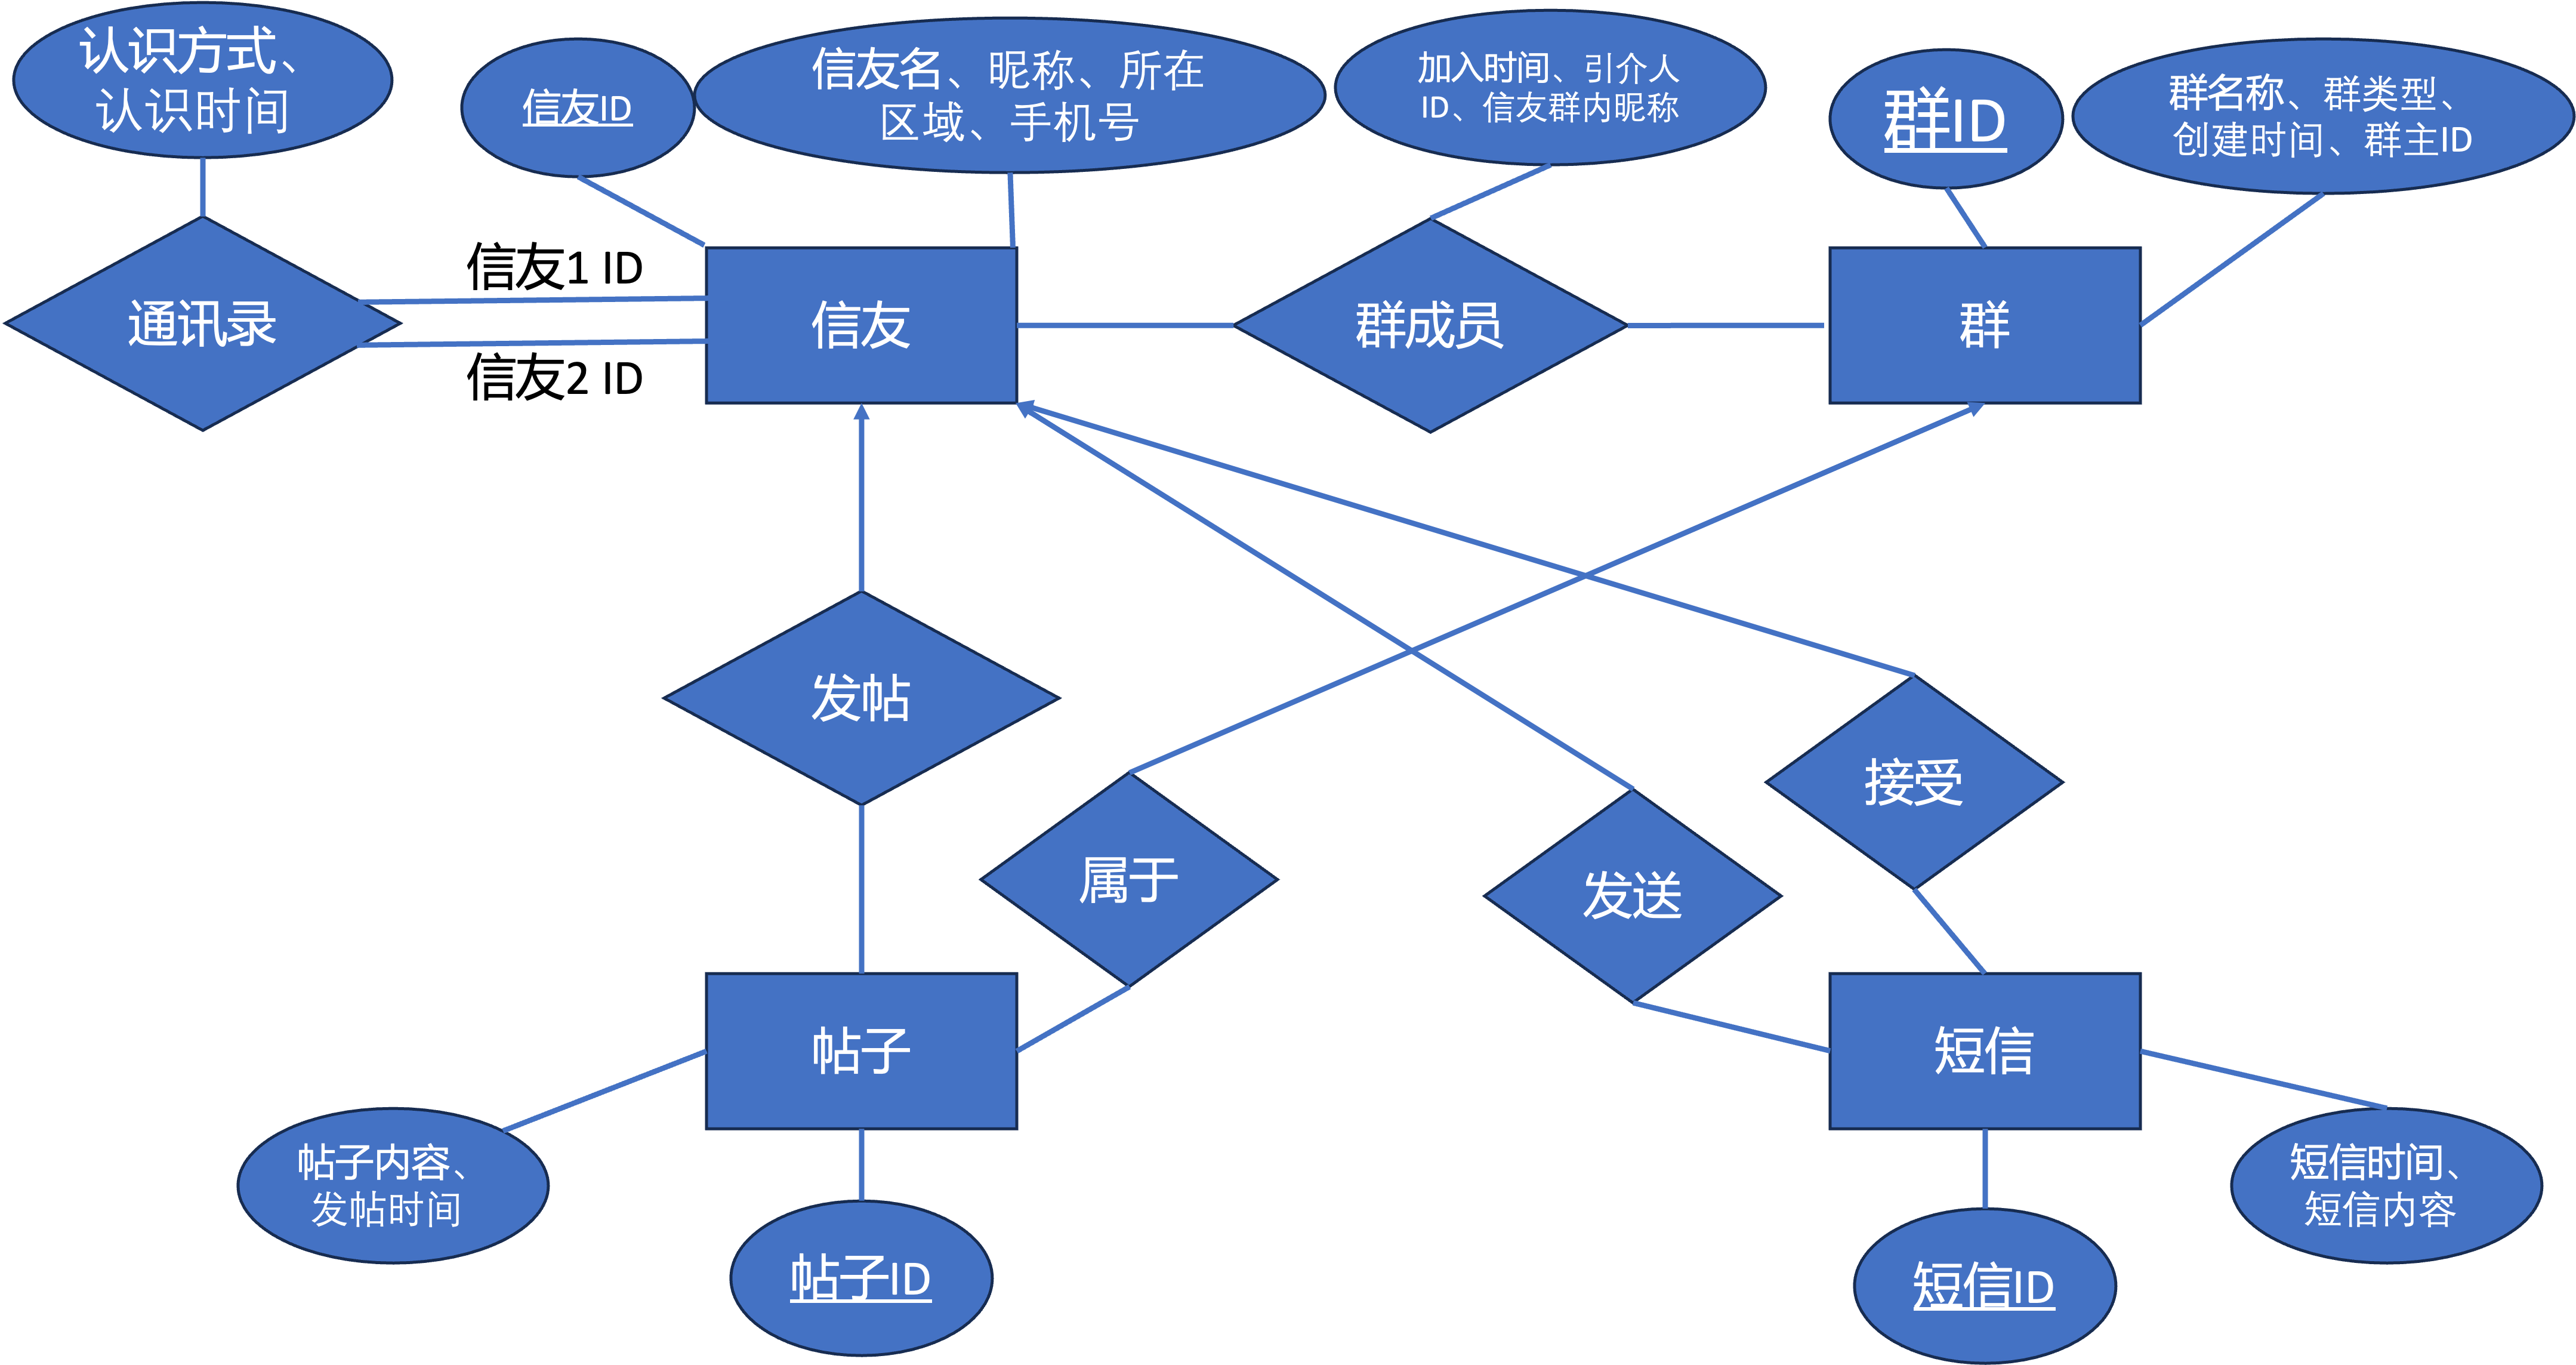
\includegraphics[width=1\textwidth]{./figs/4.png}
  \caption{题4的E-R图}
\end{figure}
\end{proof}

\begin{problem}
对于一个论文评审数据库,记录有如下信息:
\begin{enumerate}
  \item[\ding{172}] 论文有\uline{论文ID}、标题、摘要、所属主题(一个)、作者(多位)、通讯作者(一位)
  \item[\ding{173}] 作者有\uline{作者ID}、姓名、投稿论文(多篇)
  \item[\ding{174}] 审稿人有\uline{审稿人ID}、email、所关心的主题(多个)
  \item[\ding{175}] 主题有\uline{主题ID}、名称、主持人(由一位审稿人主持)
  \item[\ding{176}] 每篇论文分配给4位审稿人,从可读性、创新性、相关性打分(1-10分)
  \item[\ding{177}] 每位审稿人生成书面意见反馈给通讯作者
\end{enumerate}
请根据以上描述,画出其ER图
\end{problem}

\begin{proof}
可以画出如下的E-R图:
\begin{figure}[H]
  \centering
  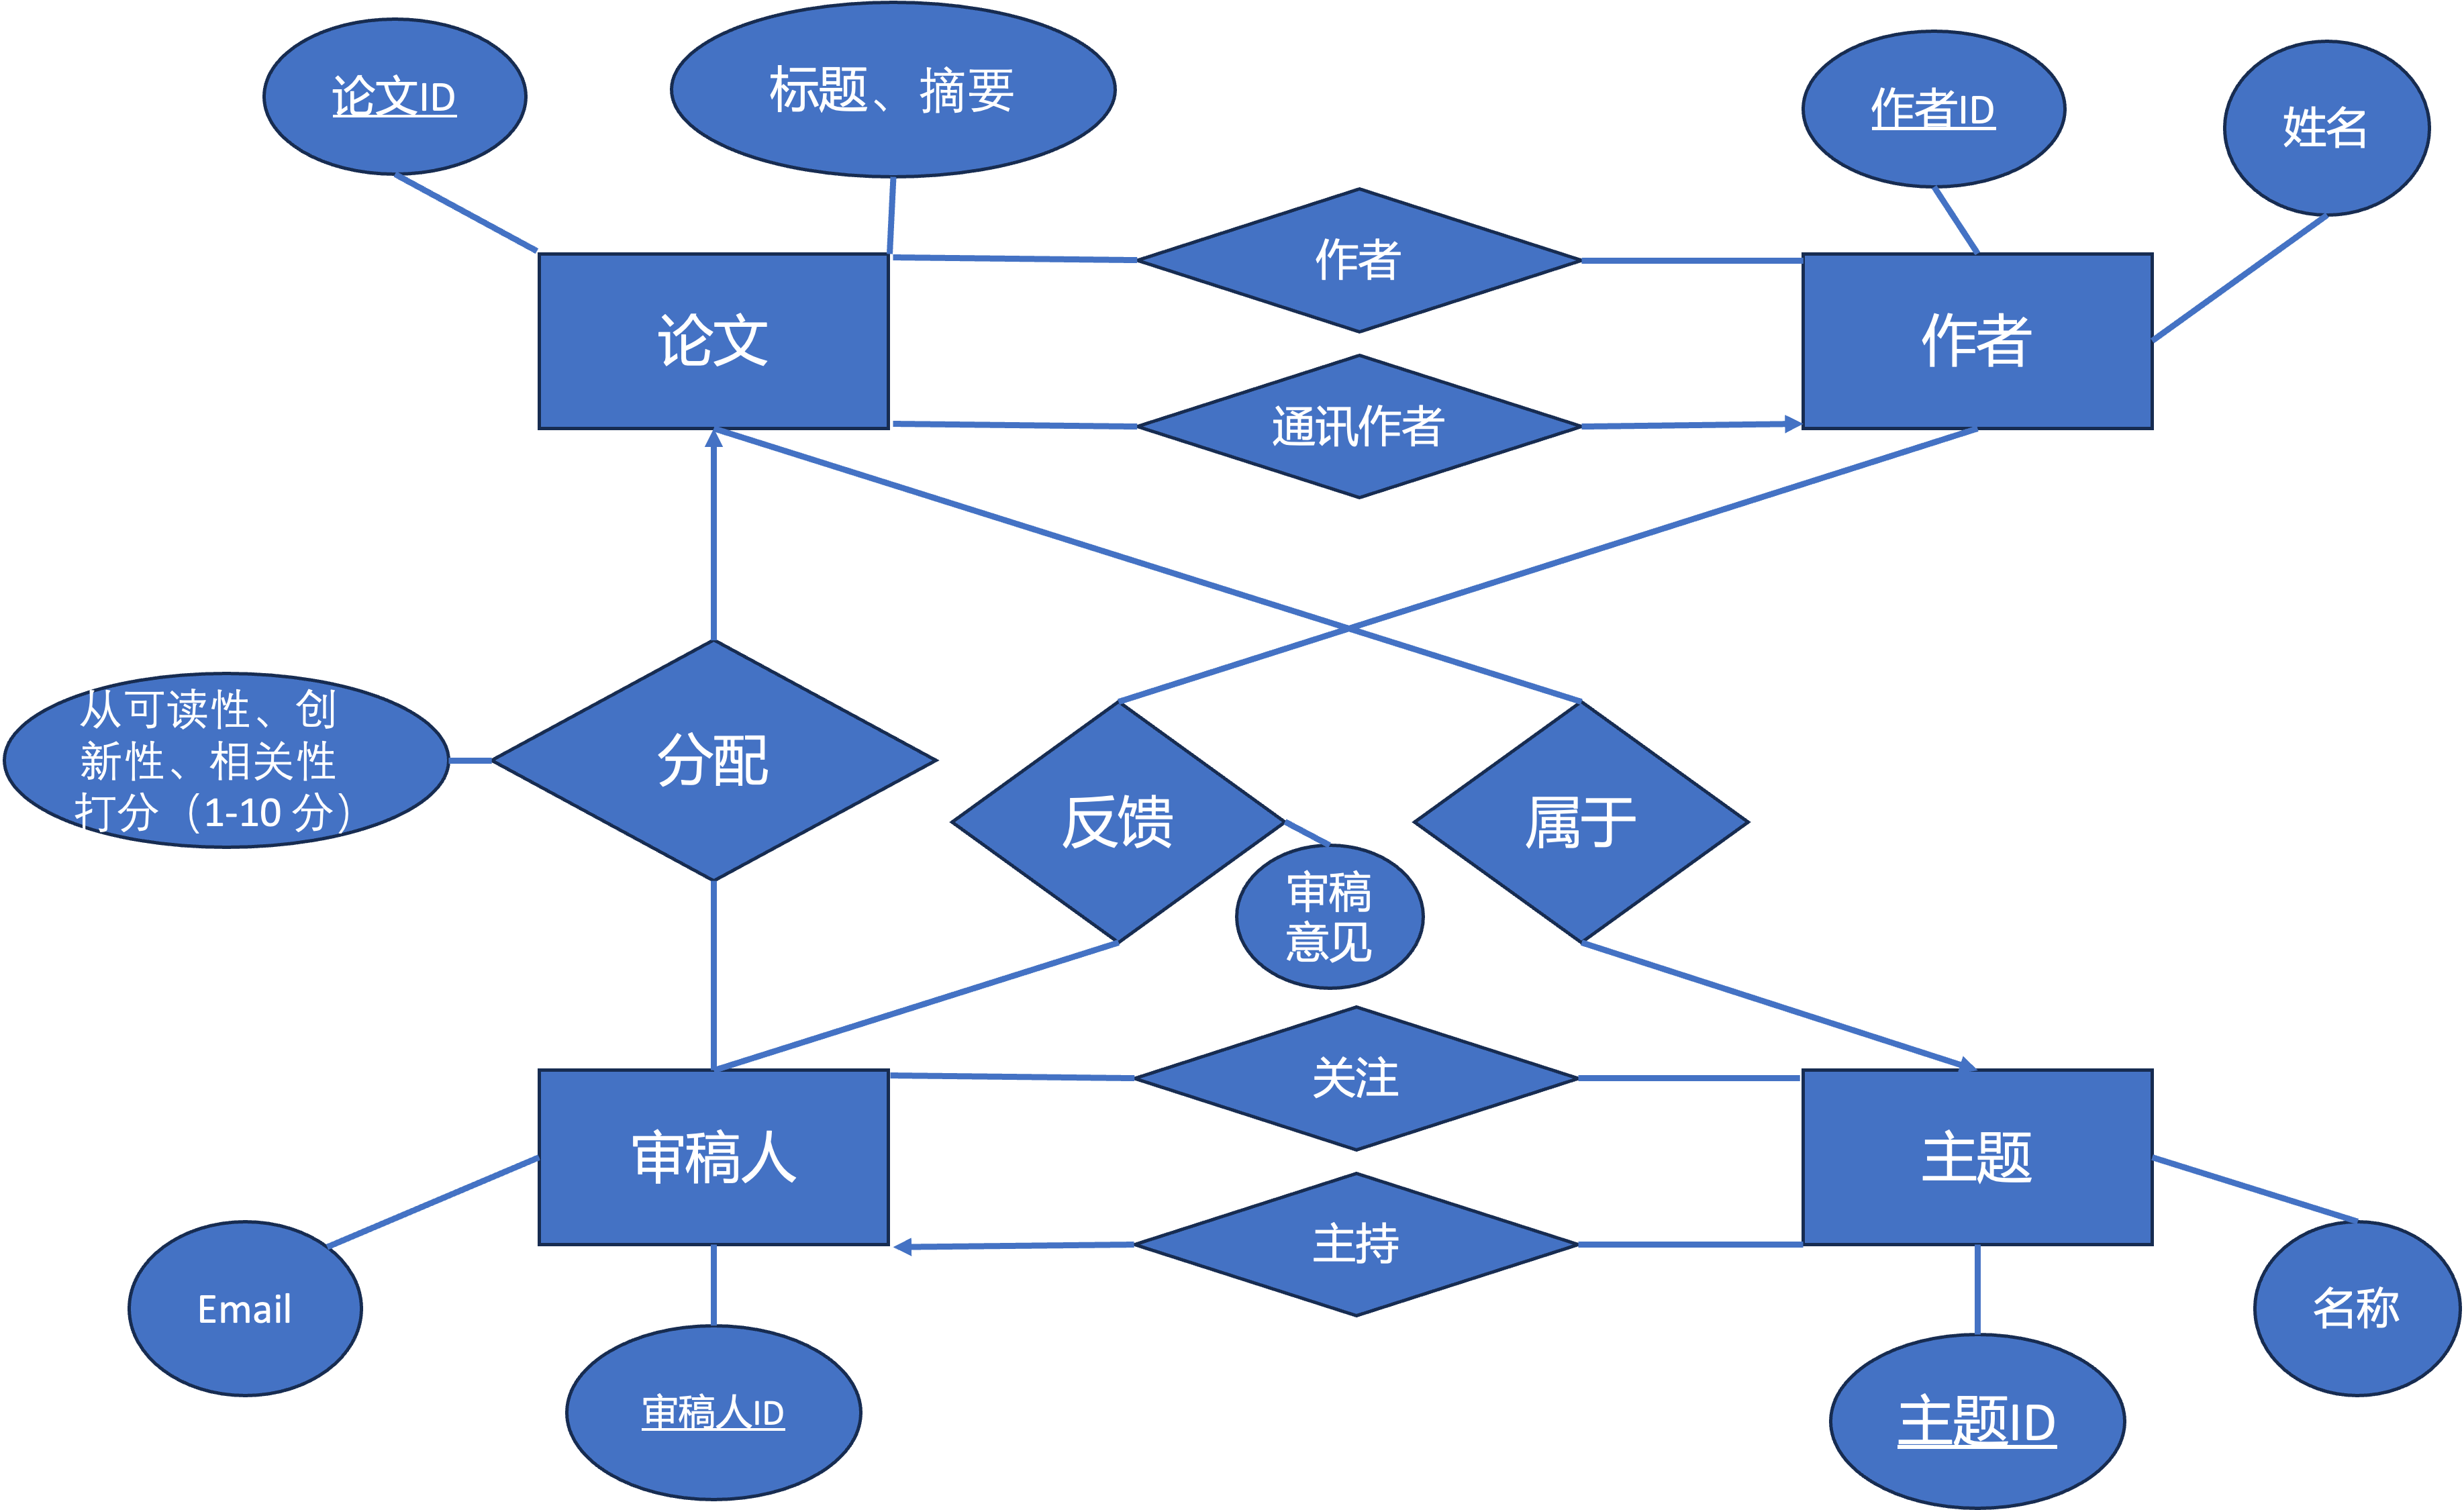
\includegraphics[width=1\textwidth]{./figs/5.png}
  \caption{题5的E-R图}
\end{figure}
\end{proof}

\begin{problem}
考察航班、航线、机场、机组、飞机、飞行员之间的业务关系,先罗列出来,尽可能地与实际情况相符,然后再画出相应的ER图

另外,MySQL自带了一个airport数据库,\href{https://downloads.mysql.com/docs/airportdb-en.a4.pdf}{这个链接}提供了相应的文档描述,同学们也可以基于它来直接完成概念建模。
airportd的表结构如下图所示:
\begin{figure}[H]
  \centering
  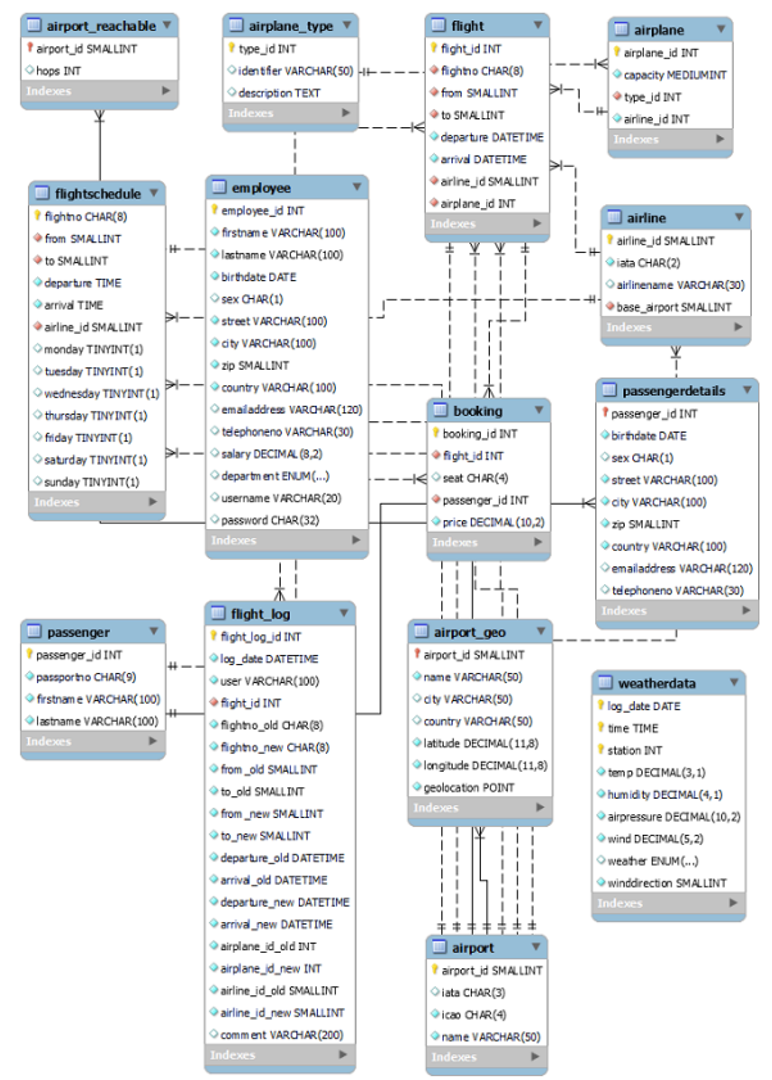
\includegraphics[width=0.4\textwidth]{./figs/6.png}
  \caption{airport数据库表结构}
\end{figure}
\end{problem}

\begin{proof}
\textbf{实体间关系}
\begin{enumerate}
  \item 航班(\uline{航班号},执飞航线号,机组编号,飞机编号,所属航空公司,起飞时间,降落时间)
  \item 航线(\uline{航线号},起飞机场,降落机场,航线长度,航线飞行时间)
  \item 机场(\uline{机场编号},机场名称,所在城市,所在国家)
  \item 机组(\uline{机组编号},飞行员编号,空乘人员编号)
  \item 飞机(\uline{飞机编号},飞机型号,所属航空公司,飞机状态)
  \item 飞行员(\uline{飞行员编号},飞行员姓名,飞行员性别,飞行员年龄,飞行员飞行时间)
\end{enumerate}

\begin{figure}[H]
  \centering
  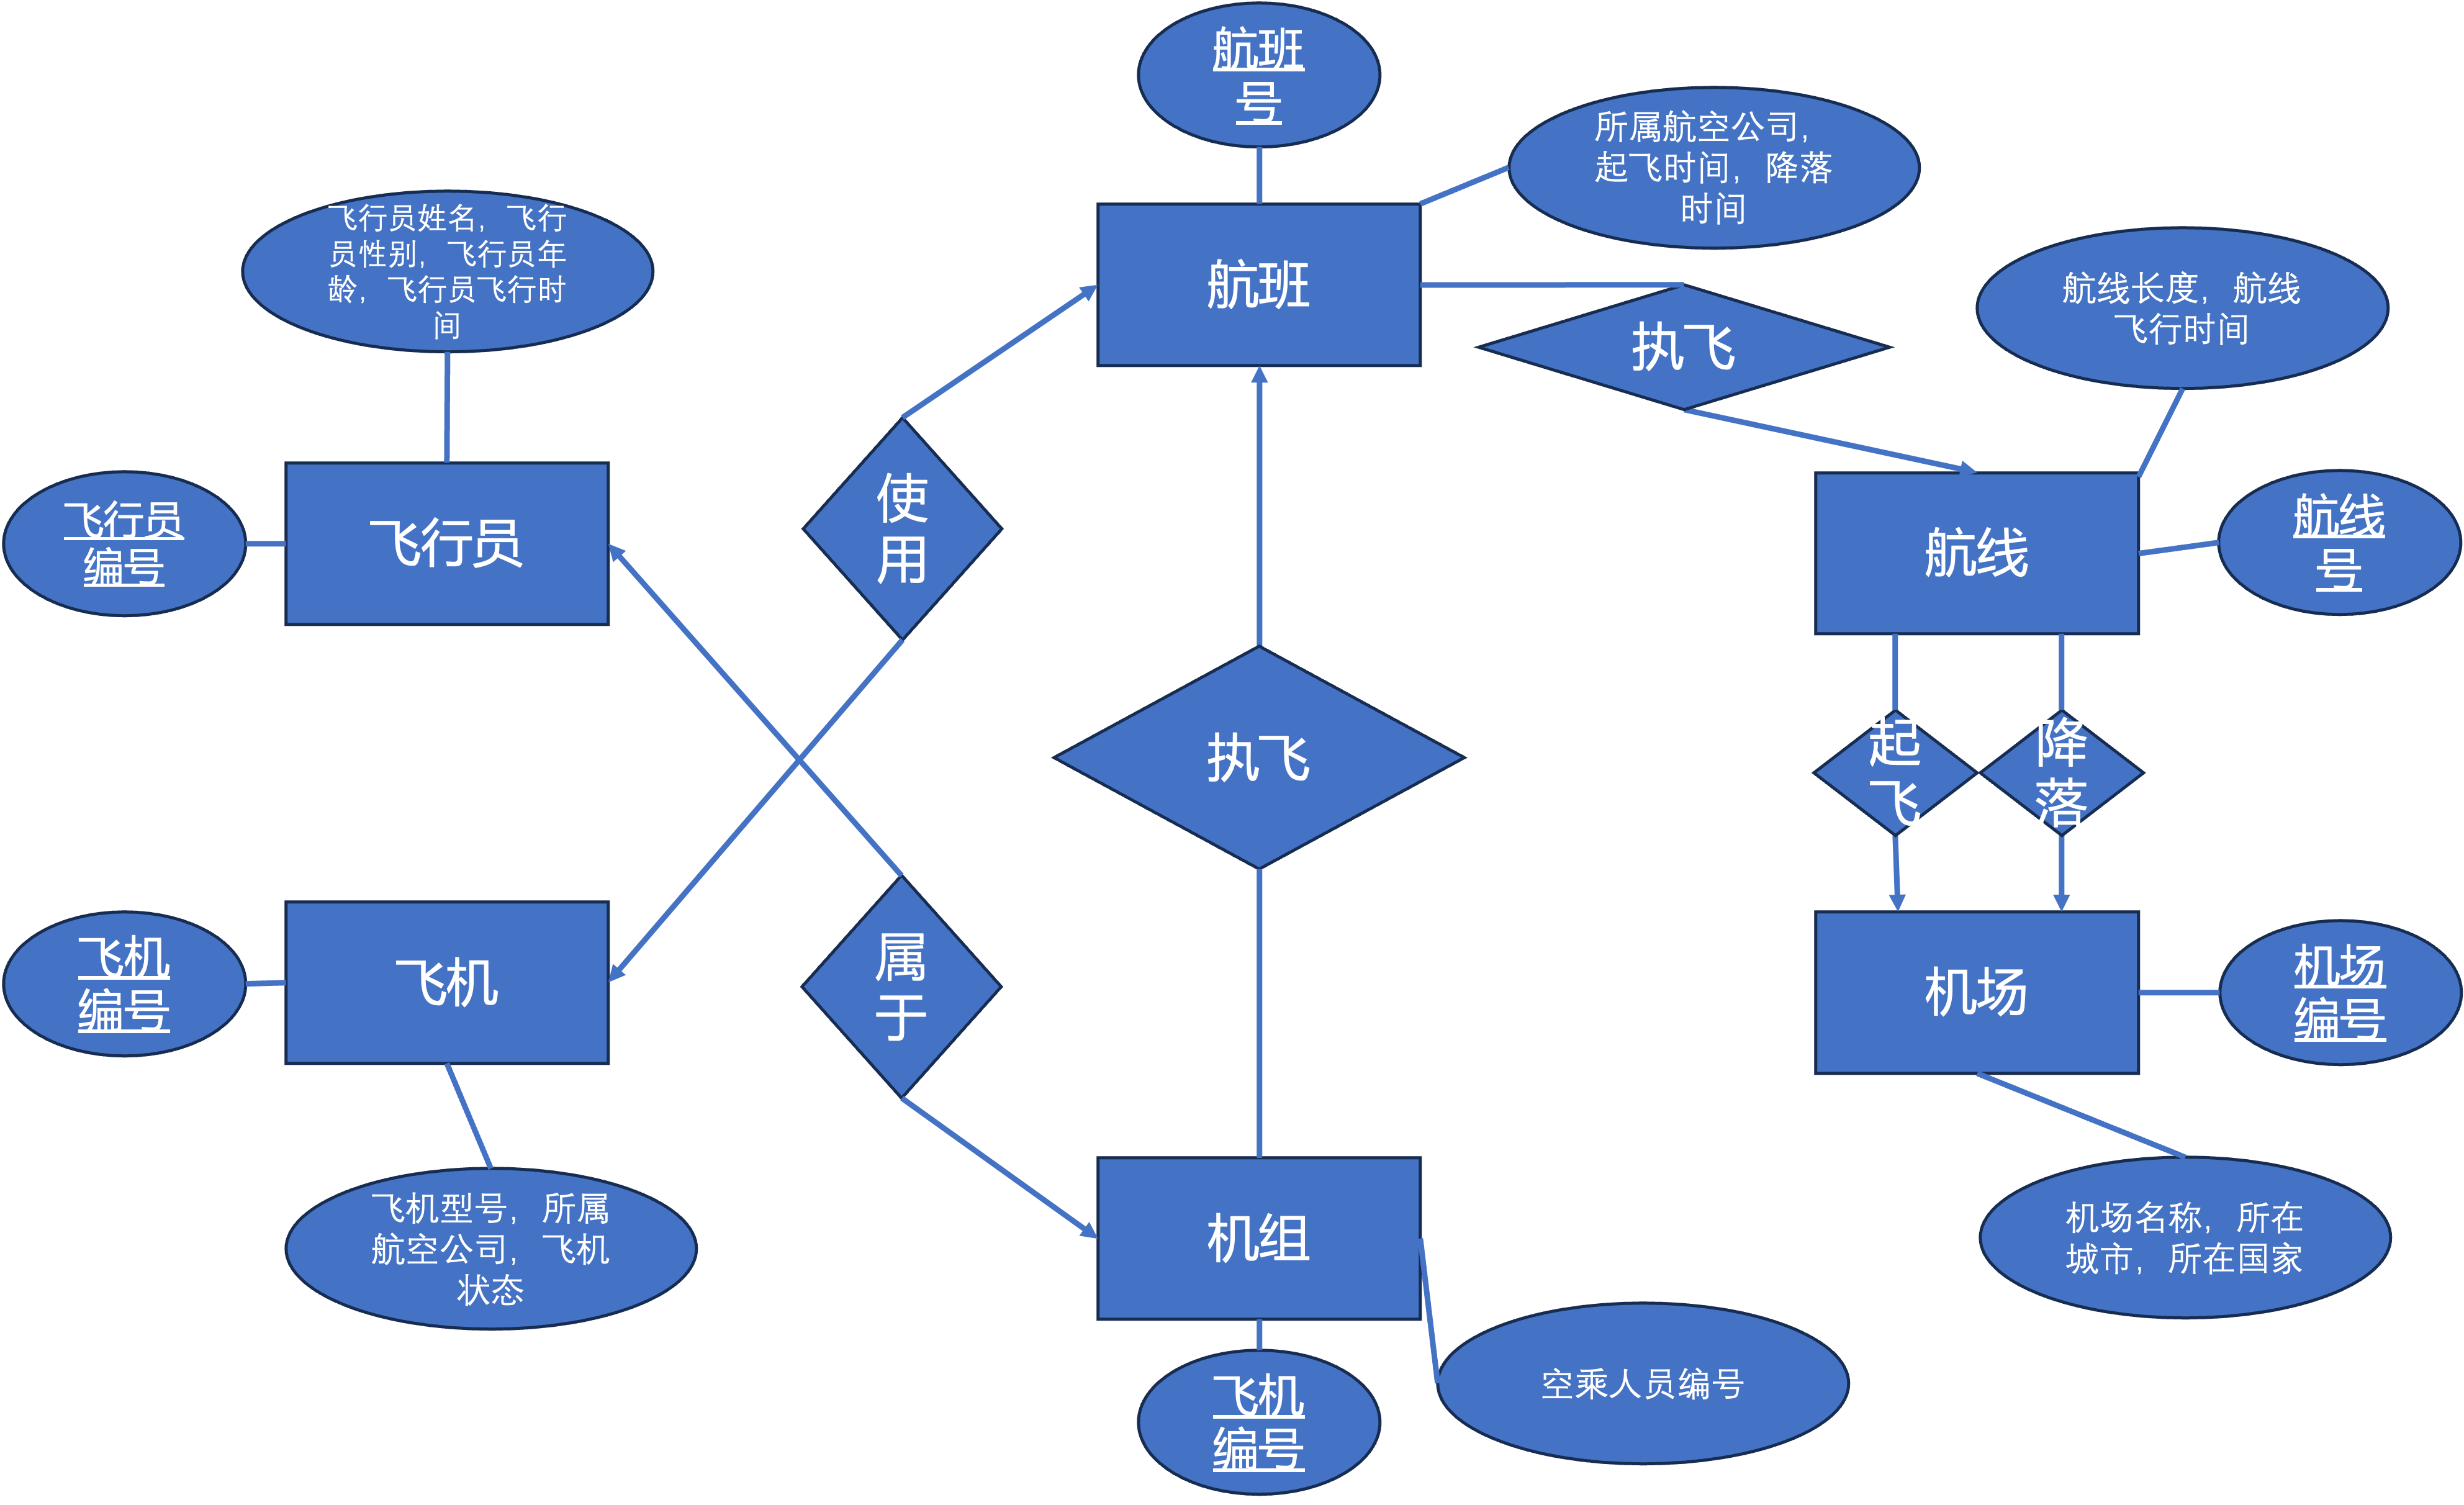
\includegraphics[width=1\textwidth]{./figs/6.1.png}
  \caption{题6的E-R图}
\end{figure}

\end{proof}

\newpage
\bibliographystyle{plain}
\bibliography{ref}


\end{document}
